\chapter{Testing \& Evaluation} \label{cha:testing}
This chapter will provide details on functionality and performance tests carried out on the completed system and will provide some analysis of results gathered through these. 

\section{Using the System}
Tests within this section will test the actual functions of the system. It will go over different features of the system and check that they all work as intended.

For all tests in this section a Raspberry Pi 4b was used to host client code, running Raspberry Pi OS Lite (with no desktop environment), which was released on December 11th 2023. The server and frontend were hosted on a Laptop with an Intel i5-12450H processor, running Fedora 39 Linux. The Raspberry Pi's hostname (visible in screenshots) is "nikpi".
\subsection{Controlling one connected device} \label{cha:testing:onedevice}
Perhaps the most obvious and basic test is to create a device, using the Rust client library, have it run on a device and to connect with that device to a running server. 

\subsubsection{Testing Setup}
A simple client was created, with two capabilities "Turn On" and "Turn Off". The callback functions attached to these capabilities would simply log to the standard output the name of the capability they are attached to. The Raspberry Pi is connected to the same Wi-Fi network as the server. The port 2302 has opened on the laptop's firewall to ensure the Raspberry Pi can make requests to the gRPC server. The Raspberry Pi is being controlled through a secure shell connection (SSH) (visible on the left side of screenshots). View figure~\ref{fig:example_config_raspi} for the exact configuration of the client.
\begin{figure}[h]
\caption{Client's configuration file}
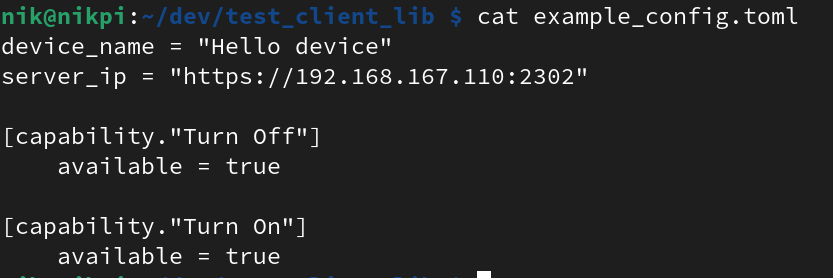
\includegraphics[width=\textwidth]{example_config_raspi}
\label{fig:example_config_raspi}
\end{figure}

\subsubsection{Testing}
Figure~\ref{fig:establish_connection_raspi} shows the successful connection and certificate exchange between the client on nikpi and the server. Note that the server ip that the client is connecting to is set within the client's configuration file (view figure~\ref{fig:example_config_raspi}). In this case the server (on the right side of figure~\ref{fig:establish_connection_raspi}) is being started with the "json-frontend" flag, as discussed within subsection~\ref{sec:chapimpl:frontend:json}, this flag is required to use the web-based frontend.
\begin{figure}[h]
\caption{Establishing a connection }
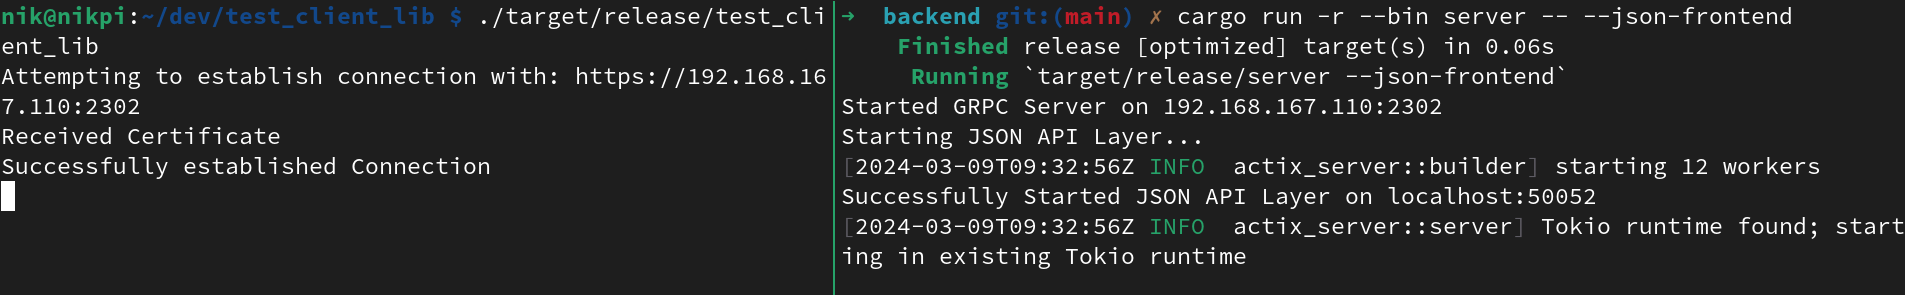
\includegraphics[width=\textwidth]{establish_connection_raspi}
\label{fig:establish_connection_raspi}
\end{figure}

The next important test is viewing the web frontend, to see that the device is correctly displayed on the frontend, with the appropriate capabilities. This can be seen in figure~\ref{fig:web_frontend_one_connected_device}, where the device, named "Hello device" (view configuration file) can be seen with it's two capabilities "Turn Off" and "Turn On". The web-frontend is being hosted by a Vite server, through using the command "npm run dev", on localhost port 5173. The frontend is being rendered by the Chromium web browser.
\begin{figure}[h]
\caption{Web Frontend with the connected device}
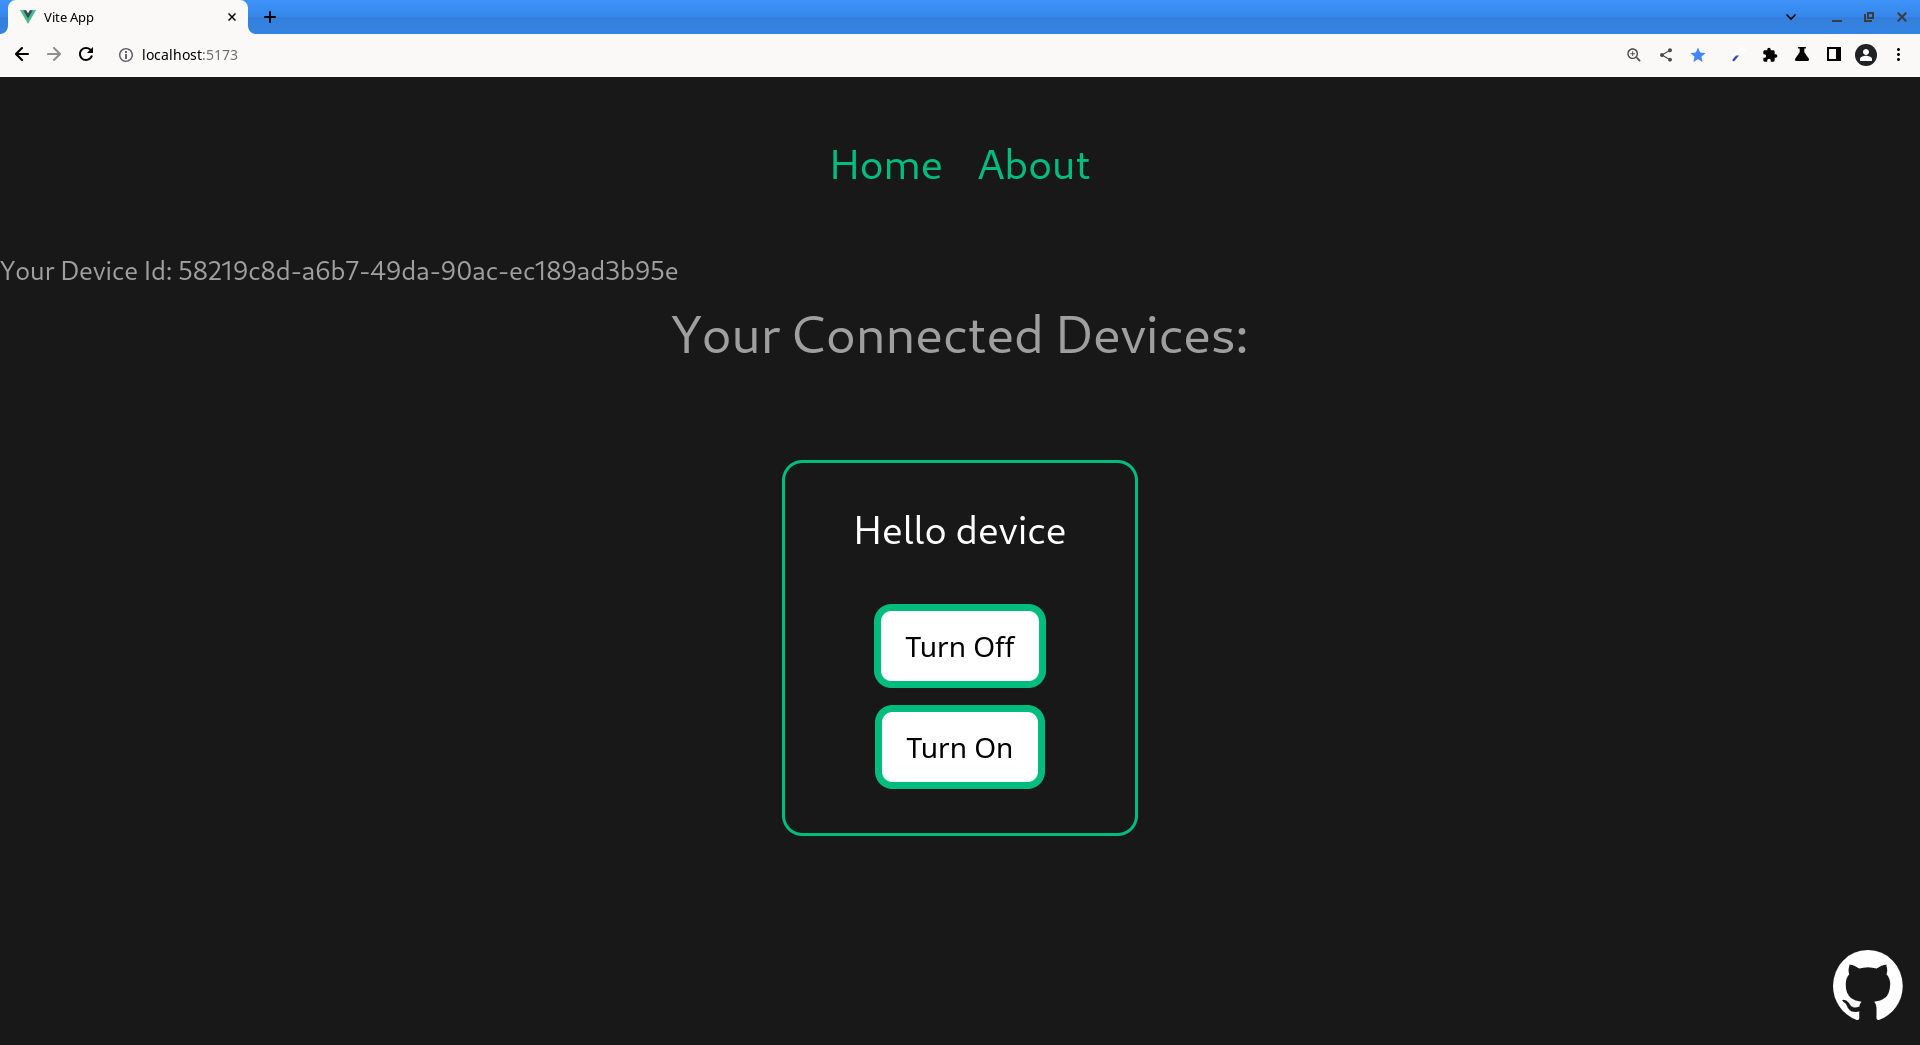
\includegraphics[width=\textwidth]{testing_web_frontend_one_device}
\label{fig:web_frontend_one_connected_device}
\end{figure}

The final test for this subsection is to attempt to trigger the two listed capabilities, by clicking the buttons. This should send a JSON packet to the JSON proxy server, which is then forwarded to the gRPC server. Once this request has been processed, the server will add it to the list of updates for the specified client. The client will then eventually poll the server and receive the update. It will then call the callback function associated with that capability. For this specific test both buttons will be clicked, starting with the "Turn Off" button, then the "Turn On Button". As shown in figure~\ref{fig:triggering_capability} this works as expected and the associated callback functions are called.
\begin{figure}[h]
\caption{Triggering capabilities}
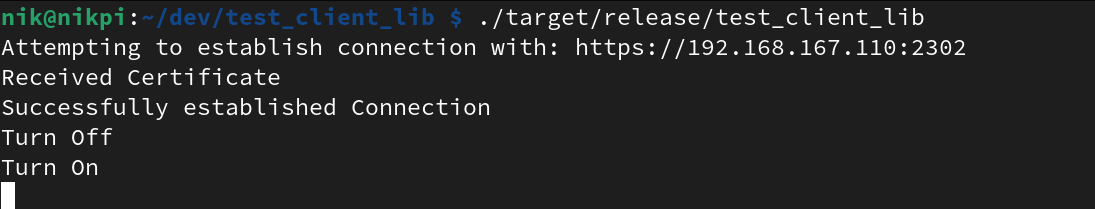
\includegraphics[width=\textwidth]{toggle_turn_on_off}
\label{fig:triggering_capability}
\end{figure}

You can view the complete code for the client used in this example in the appendix in appendix section~\ref{chap:A2:onedeviceclientlib}. Due to the simplicity of setting up a client using the NOSHP-Client library, its only 47 lines long.

\subsection{Controlling multiple connected devices}
This section will be a continuation of the last section, except that multiple devices will now be run, instead of just one. One device will still be run off the Raspberry Pi, the other devices will be run locally, on the server. They will however still be connecting to the public IP Address, not the loop-back address. Running them on the same device as the server has potential performance implications, however it is not relevant to this section, as we are simply attempting to test the functionality of the system.

\subsubsection{Testing}
One slight modification has been made to the client code in appendix section~\ref{chap:A2:onedeviceclientlib}, a print statement has been added to the main function, which prints the device name to standard output. This aids in clarity for which device is which in the screenshots. Additionally, configurations have slightly changed, with each device having uniquely named capabilities and device names, to demonstrate the frontend's ability to show different devices. The IP address they are connecting to will stay the same (the server's IP printed at startup).

\begin{figure}[h]
\caption{Establishing Connection with four devices}
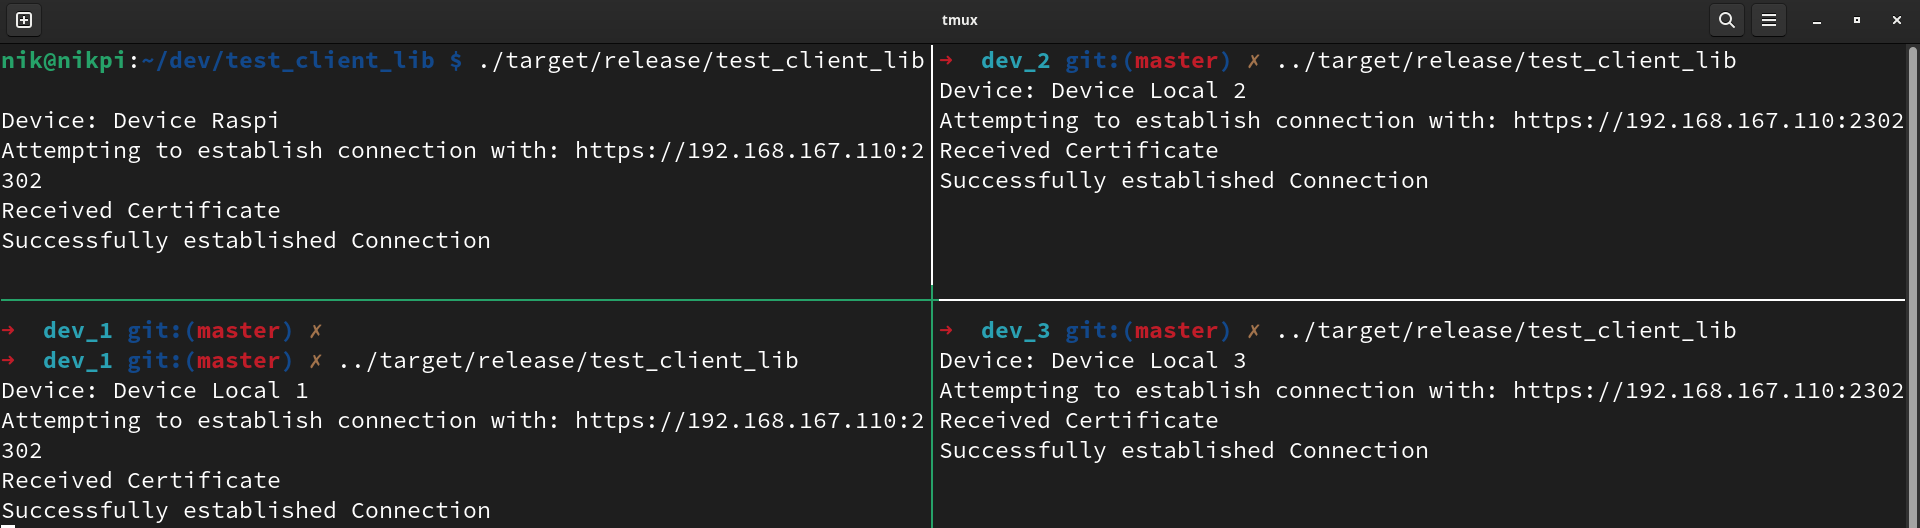
\includegraphics[width=\textwidth]{testing_four_devices_connection.png}
\label{fig:four_connected_device_connection}
\end{figure}
As seen in figure~\ref{fig:four_connected_device_connection}, connecting four devices the server is no problem. All four connect, receive their certificate and print that they have successfully established their connection. The next test is to see that all are displayed properly on the frontend, with the correct device names and capability names.


\begin{figure}[h]
\caption{Web-frontend with four devices}
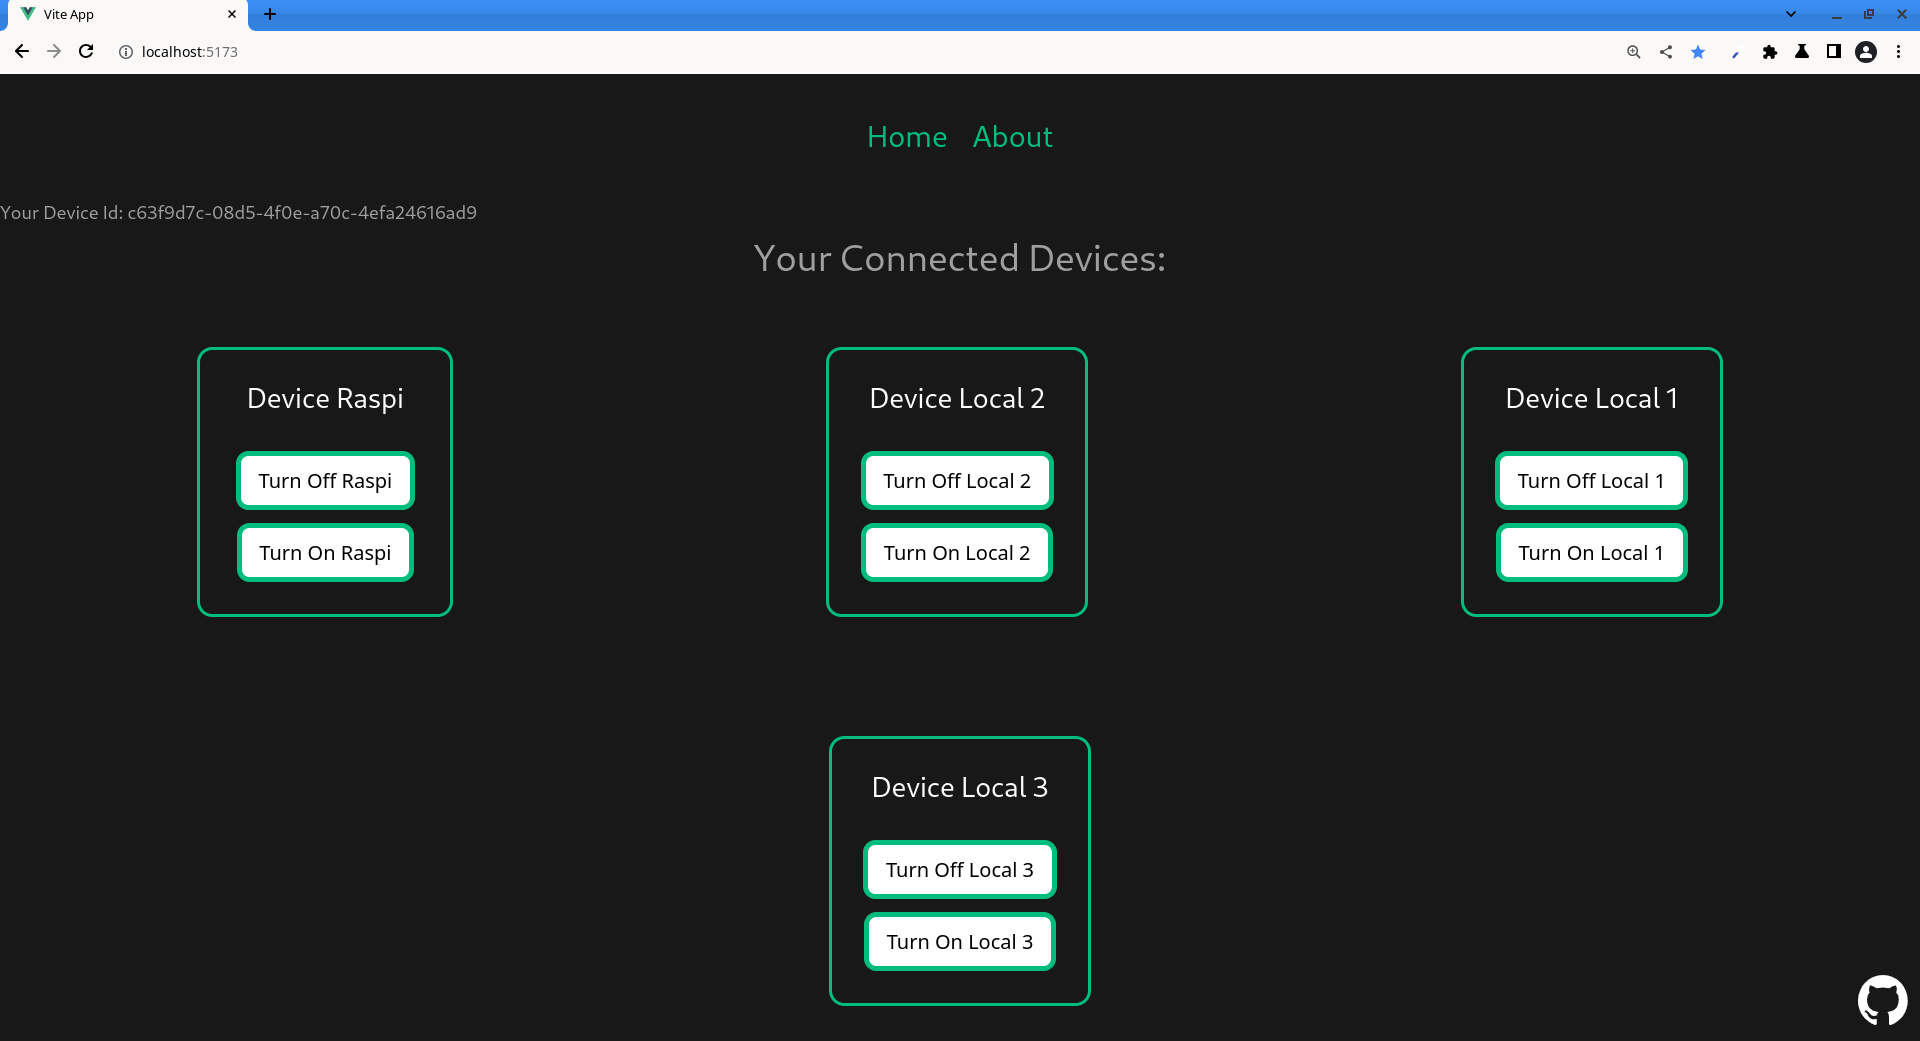
\includegraphics[width=\textwidth]{testing_four_devices_frontend.png}
\label{fig:four_connected_device_frontend}
\end{figure}
Figure~\ref{fig:four_connected_device_frontend} shows all four devices, with their correct names and capabilities displayed on the web frontend. Note that nothing has been changed about the frontend during this time, this has all been dynamically changed due to changing connected devices. Finally, we must test controlling each of the four devices. This was done by clicking every button seen on screen, from left to right and top to bottom order. The results from this can be seen in figure~\ref{fig:four_connected_device_toggle}.

\begin{figure}[h]
\caption{Triggering capabilities with four devices}
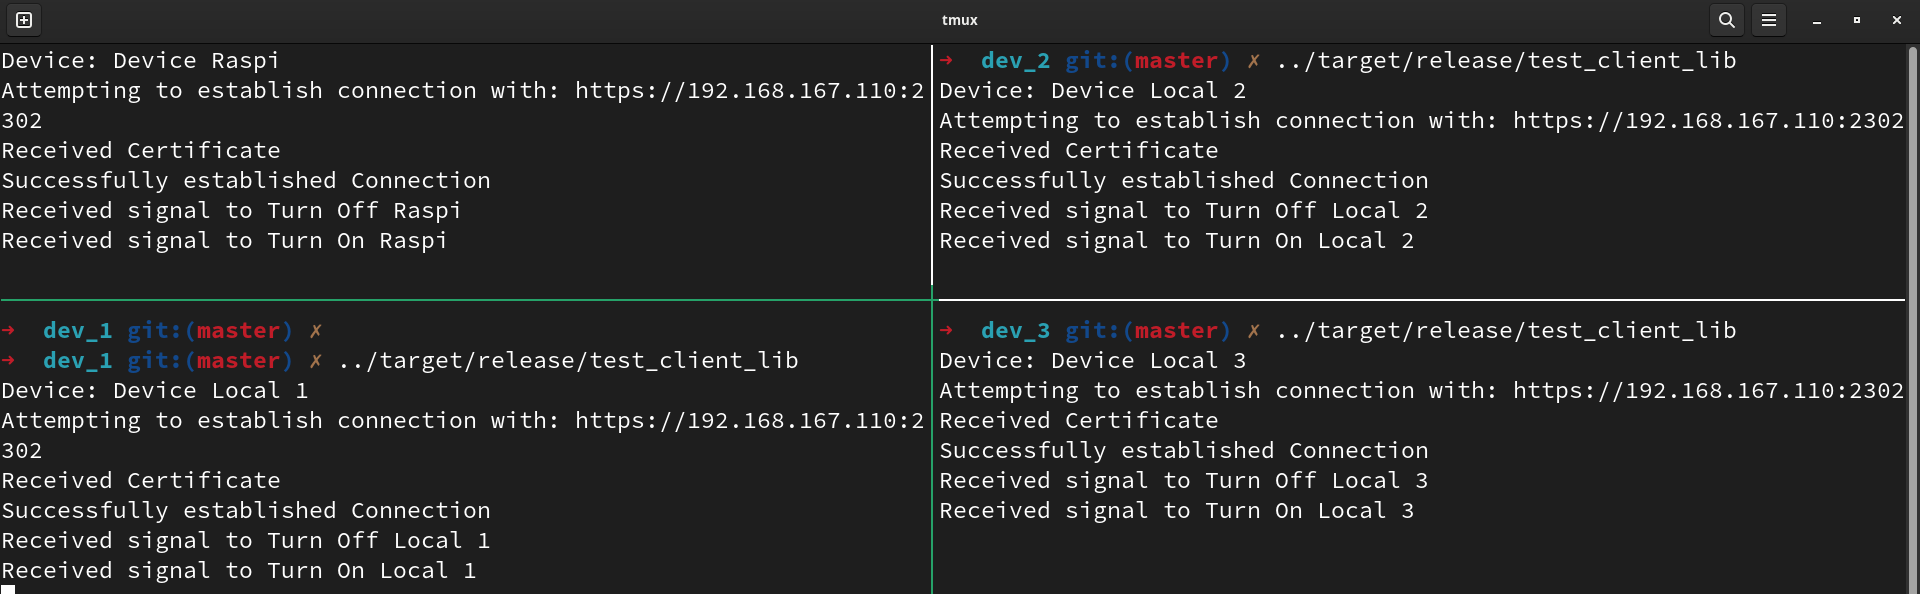
\includegraphics[width=\textwidth]{testing_four_devices_toggle.png}
\label{fig:four_connected_device_toggle}
\end{figure}
All four devices trigger their capabilities correctly. That being said, a potential issue was uncovered during this experiment. Due to latency between server and device (specifically the Raspberry Pi which was connected through Wi-Fi), packet signatures can expire before they reach the device. This can lead to lost information, as the server has already removed the update. While a somewhat rare problem, it could happen frequently on a faulty connection. An easy fix was to increase the amount of time it takes for a signature to expire, however a proper fix would for the client to send a response message, when the update has been received. The server would only delete updates when this message is received. 

\section{Performance Testing}
The main metric that was interesting for performance testing was the amount of clients the server can handle, connected at once. A secondary objective was testing the performance of the client.

\subsubsection{Additional Programs}
Gnome's "System Monitor" was used during the testing process to monitor resource usage of the server. Window's "Task Manager" was used to view the client's resource usage.

Two simple programs were constructed for this testing process. The first is a mock frontend. This frontend's Job is to act as a sort of distributed denial of service attack (DDOS) on the server, attempting to generate as many requests in a short amount of time as possible. To do this, it requests all connected devices and their capabilities. It then iterates through every connected device and sends a request to trigger all available capabilities. It repeats this process multiple times, with the amount being determined by an argument passed to the program, which is called "count". If the server has 10 clients connected to it, with two capabilities each, with the DDOS' count variable being set to 100, then \(requestAmount = 10 * 2 * 100 = 2000\). All these requests are sent as fast as the server will accept them. Each request also carries a timestamp with it, of when it was sent. This can then be measured against when the server forwards the request, to find the time it took for the server to receive, process and forward the request. These requests are sent through gRPC, so there is no added delay from the JSON http-proxy to take into account. View the code for this DDOS attack below (from \textit{\textbf{testing/ddos\_noshp\_server/src/main.rs}}):
\begin{lstlisting}[language=Rust, style=boxed, showstringspaces=false]{}
    println!("Starting DDOS Attack");
    for _ in 0..args.count {
        println!("finished iteration");
        let devices = 
            get_connected_devices(
                &device_id, 
                &mut registration_client
            )
            .await
            .unwrap();

        for device in devices.iter() {
            for capability in device.capabilities.iter() {
                if capability.available {
                    control_client.control_device(
                        DeviceControlRequest {
                            capability: capability
                                .capability.clone(),
                            device_uuid: device
                                .device_uuid.clone(),
                            timestamp: get_timestamp(),
                        }
                    ).await.unwrap();
                }
            }
        }
    }
    return Ok(());
\end{lstlisting}

The second program written for these tests is a simple client implementation, that uses the NOSHP\_client library to spawn clients, each running on its own thread. It will spawn the amount of clients specified through a command line argument, stored in the "count" variable. View the code for this second program below (from \textit{\textbf{testing/spawn\_noshp\_clients/src/main.rs}}):
\begin{lstlisting}[language=Rust, style=boxed, showstringspaces=false]{}
for i in 0..args.count {
    let mut config = config.clone();
    config.device_name += &i.to_string();
    let handle = tokio::spawn(async move {
        let client_handler = NoshpClient::new()
            .add_callback("Turn On", 
                Box::new(turn_on_led))
            .add_callback("Turn Off", 
                Box::new(turn_off_led))
            .run(config)
            .await
            .unwrap();
    });
    thread_handles.push(handle);
}

for handle in thread_handles {
    handle.await.unwrap();
}
\end{lstlisting}

\subsubsection{Testing Methodology}
The clients and server were separated between two computers. This decision was made to ensure fair results. The server was run on a laptop, with an Intel i5-12450H processor, 16 GB of memory and running Fedora 39 Linux. The laptop was plugged into power and was set to performance mode. Clients were run on a desktop, through a Windows sub-system for Linux 2 (WSL2) installation of Ubuntu 20.04 LTS. The desktop had an AMD Ryzen-7700x processor at stock settings, with 32 GB of memory. WSL2 had access to all 16 logical processes (8 cores) and 16 GB of memory. The laptop and desktop were connected through a 100 Mb/s Wi-Fi connection. 

The main metric that was being measured during this testing process was the processing time of the server. How long, on average, would it take for the server to process a request from the frontend under different loads? To test this, the time a request was sent from the frontend was taken, which was then measured against the time the request was forwarded to the client.
    
An important factor to keep in mind during this experiment was the polling rate of the client. A client will poll the server for new updates every 500ms, meaning that even if the time to process a packet is 0ms, the average response time of the server would still be 250ms, as the packet does not send the request until polled by the client. This means that optimal results from this experiment should trend towards that average, with anything above 250ms being of concern.

\subsubsection{Test Setup}
Five amount of clients were tested: 1, 10, 100, 500 and 700 clients connected to the server simultaneously. More than this were also attempted, however at above 700 clients the desktop's Linux operating system stopped being able to spawn new clients, citing OS error 24 "Too many open files". View appendix section~\ref{chap:A2:oserror} to see an example of the error. It was therefore decided that 700 clients would be the upper limit of this test. That being said, 700 clients is far more than what will likely be connected to the system at one time. Each client in this test had two active capabilities, which would print to the standard output.

To simulate a high server load, the program simulating a DDOS attack (described above) was used. This program ran with 100 iterations for every number of clients, triggering each of their two capability. Each client would therefore have 200 requests, as fast as the server could receive them. Keeping the iterations the same for every run gave an advantage to the smaller number of clients, as not only did the server have to deal with fewer clients, but also less total requests. That being said it is a worthwhile trade-off, as this is mainly a test of how many requests the server can handle, before slowing down. The number of clients mainly has an impact on memory usage, not on performance. In this case that main way of scaling requests was simply to increase clients. Additionally, it also gives the server an advantage, due to the way the server code is written. Each client can be accessed independently, at the same time (by multiple cores or threads). However, due to the use of mutual exclusion, each client could only be accessed from one thread at a time. So having more requests, with less clients, would actually have a larger impact on server performance than the other way around.

\subsubsection{Results} \label{chap:testing:results}
\begin{center}
    \textbf{Table of Test Results:} 
\begin{tabular}{ |c|c|c| } 
 \hline
 Clients / Total Requests & Mean Response Time (ms) & Median Response Time (ms)\\ 
 \hline
 1 / 200 & 378.3333333 & 379 \\ 
 \hline
 10 / 2,000 & 181.6666667 & 133.3333333 \\ 
 \hline
 100 / 20,000 & 244.6666667 & 240.6666667 \\ 
 \hline
 500 / 100,000 & 252.3333333 & 250.6666667 \\ 
 \hline
 700 / 140,000 & 251 & 247.3333333 \\ 
 \hline
\end{tabular}
\end{center}

\begin{figure}[h]
\caption{Performance Test Results Charted}
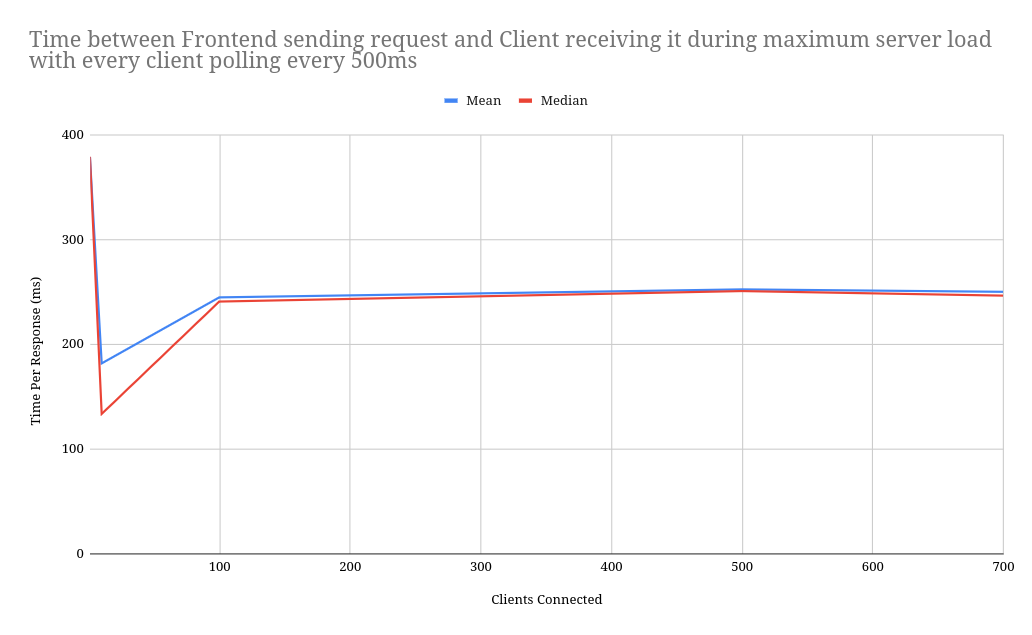
\includegraphics[width=\textwidth]{test_results_chart.png}
\label{fig:test_results_chart}
\end{figure}

Each test was run a total of three times, the mean of all three results were taken as the value for each amount of clients. All experiment results can be found in the testing folder of the repository, along with scripts for calculating mean and medians of the files.

As described above, the expected mean response time was 250ms, due to the 500ms polling rate. This is clearly reflected in the data, with the larger amount of clients trending the number. Especially the tests with 100, 500 and 700 clients there is a clear trend towards that value, with the tests with 1 and 10 clients having a very small sample size of clients, that could influence these results. That is most likely why the average response processing time of one client was the longest, due to when the one client polls the server in relation to when the request was sent massively influencing these results. What this result for one client most likely means, is that on average it polled for updates 378.3 ms after a request was sent.

\begin{figure}[h]
\caption{Server CPU load during testing with 700 clients}
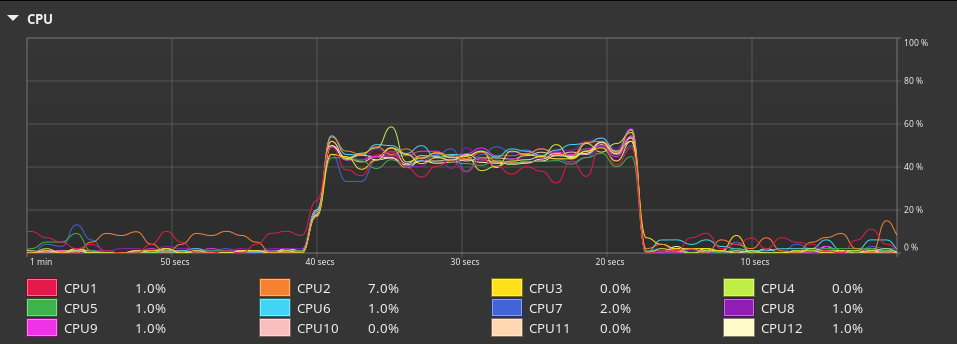
\includegraphics[width=\textwidth]{server_cpu_load.png}
\label{fig:server_cpu_load}
\end{figure}

These test results clearly show that 700 clients are not enough to create a significant enough load on the server, that it would start struggling to process packets. This is a good result, as the server is running on mid-range, laptop hardware. Additionally, realistically very few users of the software would have a need of 700 clients running on the server, especially while receiving 140,000 requests (that's nearly 7000 requests per second, seeing as the test took just over 20 seconds to run). It however does give a good indication of how the software might run on less powerful hardware.

Figure~\ref{fig:server_cpu_load} shows the CPU load during the test with 700 clients. There is a significant spike around -40 seconds, when the requests started to flood in, then the load decreases again around -18 seconds, when the server is done processing the requests. Here we can see that all CPU cores/logical processes are under load during this time, which means the concurrent handling of requests is working as intended. We can also see that the maximum load it reaches is under 60 percent. This indicates that there is still room to add more clients, especially if one factors is in that server is also simultaneously running the DDOS attack, which would create additional load. These values were captures using the Gnome "System Monitor" application.

\section{Conclusions from Testing}
One major issue was discovered while performance testing the server. The simulated clients were run on a different machine than the usability testing, for performance reasons. Specifically, this machine was running the Windows operating system. While the server accepts Unix time-stamps as timestamps, which means timezones should not matter, the time on individual machines can vary by milliseconds, to a few seconds, simply due to clock drift. Due to this fact, the Windows computer's clock had drifted into the future by milliseconds which lead to the time check not working for signature checks. As the client's time was ahead of the server's time, this lead to the simple calculation to check a packets age to return negative numbers, marking every packet as invalid. The performance tests were run with this time check disabled. This issue has since been fixed, by taking the absolute value of the difference in times, meaning the time check should work, even with slightly mismatched times.

Overall, testing was a resounding success. During performance testing, the client software was able to build first try, with no tinkering, on a machine that had never run it before. The machine was able to connect to the server with no changes needing to be made, even though it was a Windows machine (the client was however running through WSL2). Performance results are very good, with headroom on the server to accept more than 700 clients and thousands of requests per second, even on a mid-range laptop processor. Usability testing showed that the web frontend and client works exactly as expected, with multiple clients, from different sources, being able to connect to the server at one time.
